
\synctex = 1



\documentclass[10pt]{beamer}
\usetheme{metropolis}
\usepackage{CJKutf8}
\usepackage{appendixnumberbeamer}
%\usepackage{python}
%\usepackage[T1]{fontenc}
%\usepackage[utf8]{inputenc}

%\usepackage{amsthm,amsfonts,amssymb,amsmath,amsxtra}
\usepackage{mathrsfs}
\usepackage{booktabs}
\usepackage[scale=2]{ccicons}
%%%patricks
%
%\usepackage{pst-node}
%\usepackage{pst-coil}
%\usepackage{pst-func}
%\usepackage{auto-pst-pdf}
%\usepackage{pstricks-add}

%%%%
\usepackage{tikz}
\usetikzlibrary{positioning}
\usetikzlibrary{quotes,angles}
\usetikzlibrary{calc}
%\pgfplotsset{compat=1.17}
%\usetikzlibrary{matrix}
%\usepackage{pgfplots}
%\usepgfplotslibrary{dateplot}
\usetikzlibrary{patterns,arrows,decorations.pathreplacing,shapes.geometric}
\usepackage{xspace}
\usepackage{unicode-math}
\usepackage{qrcode}
\usepackage{colortbl}
\usepackage{pdftexcmds}% So I can use switch cases
%\usepackage{xcolor}
\newcommand{\themename}{\textbf{\textsc{metropolis}}\xspace}

\usepackage[all]{xy}
\xymatrixrowsep{1.5ex}  % Adjust the row spacing as needed
\xymatrixcolsep{0.5em}  % Adjust the column spacing as needed

\usepackage{pdfsync}
\usepackage{ytableau}
\usepackage{cancel}


\newcommand{\ignore}{}



%The document of how theorems displayed are in http://tex.stackexchange.com/questions/36278/box-around-theorem-statement

%This style https://www.overleaf.com/5717921pgtzmn
\usepackage[most]{tcolorbox}
\usepackage{chngcntr}
\usepackage{lipsum}

\usepackage{polynom}
% counters
\newcounter{definition}
\newcounter{lemma}
\newcounter{prop}
\newcounter{exa}
\newcounter{thm}
\newcounter{cor}
\counterwithin{definition}{section}
\counterwithin{lemma}{section}
\counterwithin{prop}{section}
\counterwithin{exa}{section}
\counterwithin{thm}{section}
\counterwithin{cor}{section}

\newcommand{\apple}{
\includegraphics[scale=0.08,natwidth=10,natheight=10]{Pictures/apple.png}}
\newcommand{\bigapple}{
\includegraphics[scale=0.13,natwidth=10,natheight=10]{Pictures/apple.png}}
\newcommand{\peach}{
\includegraphics[scale=0.08,natwidth=10,natheight=10]{Pictures/peach.png}}
\newcommand{\bigpeach}{
\includegraphics[scale=0.13,natwidth=10,natheight=10]{Pictures/peach.png}}
\newcommand{\bean}{
\includegraphics[scale=0.07,natwidth=10,natheight=10]{Pictures/bean.png}}
\newcommand{\sbean}{
\includegraphics[scale=0.04,natwidth=10,natheight=10]{Pictures/bean.png}}
\newcommand{\soup}{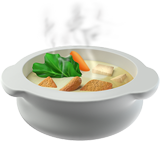
\includegraphics[scale=0.10,natwidth=10,natheight=10]{Pictures/soup.png}}
\newcommand{\ssoup}{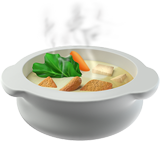
\includegraphics[scale=0.07,natwidth=10,natheight=10]{Pictures/soup.png}}
\newcommand{\bigsoup}{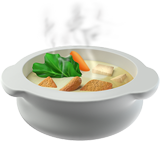
\includegraphics[scale=0.30,natwidth=10,natheight=10]{Pictures/soup.png}}
\newcommand{\lemon}{
\includegraphics[scale=0.08,natwidth=10,natheight=10]{Pictures/lemon.png}}
\newcommand{\slemon}{
\includegraphics[scale=0.05,natwidth=10,natheight=10]{Pictures/lemon.png}}
\newcommand{\biglemon}{
\includegraphics[scale=0.13,natwidth=10,natheight=10]{Pictures/lemon.png}}
\newcommand{\leaf}{
\includegraphics[scale=0.08,natwidth=10,natheight=10]{Pictures/leaf.png}}
\newcommand{\sleaf}{
\includegraphics[scale=0.05,natwidth=10,natheight=10]{Pictures/leaf.png}}
\newcommand{\milk}{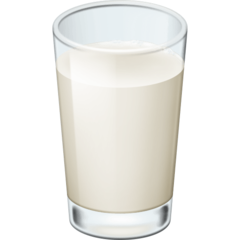
\includegraphics[scale=0.07,natwidth=10,natheight=10]{Pictures/milk.png}}
\newcommand{\smilk}{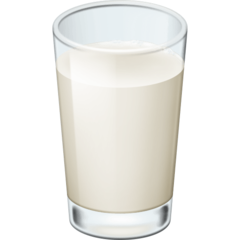
\includegraphics[scale=0.04,natwidth=10,natheight=10]{Pictures/milk.png}}
\newcommand{\coffee}{
\includegraphics[scale=0.10,natwidth=10,natheight=10]{Pictures/coffee.png}}
\newcommand{\scoffee}{
\includegraphics[scale=0.07,natwidth=10,natheight=10]{Pictures/coffee.png}}
\newcommand{\carrot}{
\includegraphics[scale=0.11,natwidth=10,natheight=10]{Pictures/carrot.png}}
\newcommand{\bigcarrot}{
\includegraphics[scale=0.15,natwidth=10,natheight=10]{Pictures/carrot.png}}
\newcommand{\cola}{
\includegraphics[scale=0.08,natwidth=10,natheight=10]{Pictures/cola.png}}
\newcommand{\scola}{
\includegraphics[scale=0.05,natwidth=10,natheight=10]{Pictures/cola.png}}
\newcommand{\tea}{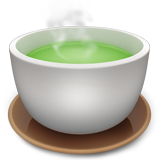
\includegraphics[scale=0.08,natwidth=10,natheight=10]{Pictures/tea.png}}
\newcommand{\stea}{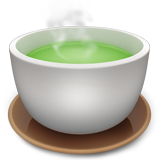
\includegraphics[scale=0.05,natwidth=10,natheight=10]{Pictures/tea.png}}
\newcommand{\teaa}{
\includegraphics[scale=0.03,natwidth=10,natheight=10]{Pictures/teaaa.jpg}}
\newcommand{\cow}{
\includegraphics[scale=0.08,natwidth=10,natheight=10]{Pictures/cow.png}}
\newcommand{\orange}{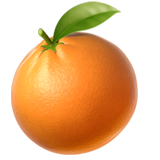
\includegraphics[scale=0.09,natwidth=10,natheight=10]{Pictures/orange.png}}
\newcommand{\bento}{
\includegraphics[scale=0.09,natwidth=10,natheight=10]{Pictures/bento.png}}
\newcommand{\sbento}{
\includegraphics[scale=0.04,natwidth=10,natheight=10]{Pictures/bento.png}}
\newcommand{\bigbento}{
\includegraphics[scale=0.13,natwidth=10,natheight=10]{Pictures/bento.png}}
\newcommand{\money}{
\includegraphics[scale=0.09,natwidth=10,natheight=10]{Pictures/money.png}}
\newcommand{\buxie}{
\includegraphics[scale=0.05,natwidth=10,natheight=10]{Pictures/buxie.png}}
\newcommand{\no}{
\includegraphics[scale=0.13,natwidth=10,natheight=10]{Pictures/no.png}}
\newcommand{\think}{
\includegraphics[scale=0.13,natwidth=10,natheight=10]{Pictures/think.png}}
\newcommand{\question}{
\includegraphics[scale=0.13,natwidth=10,natheight=10]{Pictures/question.png}}
\newcommand{\tear}{
\includegraphics[scale=0.13,natwidth=10,natheight=10]{Pictures/tear.png}}
\newcommand{\boss}{
\includegraphics[scale=0.13,natwidth=10,natheight=10]{Pictures/boss.png}}
\newcommand{\homework}{
\includegraphics[scale=0.13,natwidth=10,natheight=10]{Pictures/homework.png}}
\newcommand{\sinister}{
\includegraphics[scale=0.13,natwidth=10,natheight=10]{Pictures/sinister.png}}
\newcommand{\sleep}{
\includegraphics[scale=0.13,natwidth=10,natheight=10]{Pictures/sleep.png}}
\newcommand{\answer}{
\includegraphics[scale=0.13,natwidth=10,natheight=10]{Pictures/answer.png}}
\newcommand{\hi}{
\includegraphics[scale=0.6,natwidth=10,natheight=10]{Pictures/hi.png}}
\newcommand{\spy}{
\includegraphics[scale=0.04,natwidth=10,natheight=10]{Pictures/spy.png}}
\newcommand{\police}{
\includegraphics[scale=0.2,natwidth=10,natheight=10]{Pictures/police.png}}
\newcommand{\case}{
\includegraphics[scale=0.1,natwidth=10,natheight=10]{Pictures/box.png}}
\newcommand{\remote}{
\includegraphics[scale=0.05,natwidth=10,natheight=10]{Pictures/remote.png}}
\newcommand{\wifi}{
\includegraphics[scale=0.05,natwidth=10,natheight=10]{Pictures/wifi.png}}
\newcommand{\man}{
\includegraphics[scale=0.1,natwidth=10,natheight=10]{Pictures/man.png}}
\newcommand{\bow}{
\includegraphics[scale=0.08,natwidth=10,natheight=10]{Pictures/bow.jpg}}
\newcommand{\house}{
\includegraphics[scale=0.13,natwidth=10,natheight=10]{Pictures/house.png}}
\newcommand{\convey}{\includegraphics[scale=0.13,natwidth=10,natheight=10]{Pictures/convey.jpg}}
\newcommand{\drawer}{\includegraphics[scale=0.13,natwidth=10,natheight=10]{Pictures/drawer.png}}
\newcommand{\book}{\includegraphics[scale=0.13,natwidth=10,natheight=10]{Pictures/book.png}}
\newcommand{\rbook}{\includegraphics[scale=0.013,natwidth=10,natheight=10]{Pictures/redbook.png}}
\newcommand{\bbook}{\includegraphics[scale=0.013,natwidth=10,natheight=10]{Pictures/bluebook.png}}

\newcommand{\h}{\cellcolor{red!50}}
\newcommand{\y}{\cellcolor{yellow!50}}
\newcommand{\e}{\cellcolor{blue!50}}

\long\def\E{32}
\long\def\D#1#2\a{\BiajiBiaji{#1}#2\F\F haha \a}
\long\def\a#1#2\E#3\E{#3\D{#1}#2\E#3\E}
\long\def\BiajiBiaji#1#2\F#3\F#4\a{\edef\aa{#1}\setbeamercolor{background canvas}{bg=white}#3

\begin{frame}{#1}#2\end{frame}

 \a}%The fragile setting is made to run python code correctly.
\def\Chi#1\Chi\E{}
\long\def\aaa#1#2\aaa{\a{#1}#2\a\E\E\Chi\E}

\makeatletter

\newtcolorbox{defi}[1][]{
breakable,
enhanced,
colback=yellow!10!white,
colframe=red!75!black,
title=\definame\refstepcounter{definition}~~\arabic{definition}~~#1
}

\newtcolorbox{prop}[1][]{
breakable,
enhanced,
colback=yellow!10!white,
colframe=yellow!70!red!85!black,
title=\textbf{Proposition}\refstepcounter{prop}~~\arabic{prop}~~#1
}

\newtcolorbox{thm}[1][]{
breakable,
enhanced,
colback=yellow!10!white,
colframe=black,
title=\textbf{Theorem}\refstepcounter{thm}~~\arabic{thm}~~#1
}

\newtcolorbox{conj}[1][]{
breakable,
enhanced,
colback=yellow!20!white,
colframe=black,
title=\textbf{Conjecture}\refstepcounter{thm}~~\arabic{thm}~~#1
}


\newtcolorbox{lem}[1][]{
breakable,
enhanced,
colback=yellow!10!white,
colframe=yellow!20!red!99!blue!99!black,
title=\textbf{Lemma}\refstepcounter{lemma}~~\arabic{lemma}~~#1
}


\newtcolorbox{cor}[1][]{
breakable,
enhanced,
colback=yellow!10!white,
colframe=red!45!yellow!80!black,
title=\textbf{Corollary}\refstepcounter{cor}~~\arabic{cor}~~#1
}

\newtcolorbox{exa}[1][]{
breakable,
sharp corners=uphill,
arc=5mm,boxrule=2mm,
colback=red!2!white,
colframe=red!10!white,
}

\newtcolorbox{exap}[1][]{
breakable,
sharp corners=uphill,
arc=5mm,boxrule=2mm,
colback=blue!2!white,
colframe=blue!10!white,
}

\newtcolorbox{exapl}[1][]{
breakable,
enhanced,
%sharp corners=uphill,
arc=5mm,boxrule=2mm,
title=\textbf{\LARGE{#1}},
attach boxed title to top center={yshift=-3mm,yshifttext=-1mm},
boxed title style={size=small,colback=orange!90,colframe=red!70!black},
colback=yellow!5!white,
colframe=yellow!90!black,
}

\newtcolorbox{rem}[1][]{
breakable,
enhanced,
arc=5mm,boxrule=2mm,
title=\textbf{\LARGE{!!}},
attach boxed title to top center={yshift=-3mm,yshifttext=-1mm},
boxed title style={size=small,colback=red!95!black,colframe=red!50!black},
colback=yellow!5!white,
colframe=yellow!90!black,
}

\newtcolorbox{rema}[1][]{
breakable,
enhanced,
arc=5mm,boxrule=2mm,
title=\textbf{\LARGE{!!}},
attach boxed title to top center={yshift=-3mm,yshifttext=-1mm},
boxed title style={size=small,colback=red!95!black,colframe=red!50!black},
colback=yellow!5!white,
colframe=yellow!90!black,
}
\newtcolorbox{summ}[1][]{
breakable,
enhanced,
title=\textbf{\LARGE{Summary}},
attach boxed title to top center={yshift=-3mm,yshifttext=-1mm},
boxed title style={size=small,colback=yellow!95!black,colframe=red!50!black},
colback=yellow!5!white,
colframe=yellow!90!black,
}
\makeatother


\makeatletter
\def\t{\@tt|\em\@gobble\@ttt}
\def\em\@tt#1\em{\@tt|\em}
\def\cm\@tt#1\em#2\@ttt{
\begin{tabular}{#1}
\hline
#2
\\\hline
\end{tabular}\@gobble
}
\def\@tt#1\@ttt#2{
\@ifnextchar,{\@tt #1 & #2\\\hline\expandafter\expandafter\expandafter\@gobble\expandafter\@gobble\@gobble\@ttt}{
\@ifnextchar.{\cm\@tt|l #1 & #2\@ttt}{\@tt|l #1 & #2\@ttt}
}
}

\def\m{\@tut\@gobble\@tutt}
\def\@tut#1\@tutt#2{
\@ifnextchar,{\@tut #1 & #2\\\expandafter\expandafter\expandafter\@gobble\expandafter\@gobble\@gobble\@tutt}{
\@ifnextchar.{\begin{pmatrix}#1 &#2\end{pmatrix}\@gobble}{\@tut #1 & #2\@tutt}
}
}

\def\bm{\@tuut\@gobble\@tuutt}
\def\@tuut#1\@tuutt#2{
\@ifnextchar,{\@tuut #1 & #2\cr\expandafter\expandafter\expandafter\@gobble\expandafter\@gobble\@gobble\@tuutt}{
\@ifnextchar.{\bordermatrix{#1 &#2\cr}\@gobble}{\@tuut #1 & #2\@tuutt}
}
}





\makeatother



%\newtheorem{defi}{\color{cyan} Definition}
%\newtheorem{prop}{\color{cyan} Proposition}
%\newtheorem{cor}{\color{cyan} Corollary}
%\newtheorem{summ}{\color{cyan} Summary}
%\newtheorem{rem}{\color{cyan} Remark}
%\newtheorem{thm}{\color{cyan} Theorem}
\newtheorem{ex}[thm]{Problem}
\newtheorem{so1}{\color{blue}Solution}
\newtheorem{so2}{\color{orange}Solution(level 2)}
\newtheorem{so3}{\color{red}Solution(level 3)}
%\newtheorem{lem}{\color{cyan} Lemma}
%\newtheorem{exa}{\color{cyan} Example}


% names for the structures
\newcommand\definame{\textbf{Definition}}
\newcommand\lemmname{\textbf{Lemma}}


\newcommand{\x}[1]{\alert{\textbf{#1}}}
